\section{Conclusion and Future Work}
\label{sec:Conclusion}

%Partially processed queries are the most difficult for analysis because real set of values which can be 
%generated for query at run time and the correctness of this set values often corresponds with some 
%additional nontrivial knowledges about original system. 

%We can suppose that all values of initial queries should be correct because the original system is production system with long time history. 

%We should assume that behavior of the system is always correct. In this case any errors shows that 
%our algorithm is incorrect. On the other hand, this assumption is not always correct. 

%Firstly, developer can have some additional knowledges about semantics of code and he can guarantee that some values never 
%be got for query and this values can be incorrect. But this values can be calculated during statical 
%analysis. 

%Moreover, the dead code contained in long-lived systems can be really incorrect and the amount 
%of this code can be big. Database applications can contain legacy and test procedures which were correct 
%some times ago but not now. Dead code elimination can be useful in some of these cases, but most of 
%them should be manually investigated anyway. Detailed research of error correction and recovery 
%algorithms application for abstract parsing is required~\cite{RelaxedLALR}.
 
Semantics calculation for embedded languages is also the source of problems. The main problem is 
that we cannot guarantee semantics correctness during syntax analysis: we can get correct tree 
with incorrect semantic. Example of this situation is shown on Fig.~\ref{pic7}. In presented 
graph we can choose 2 paths which contain all variables used for query value calculation. For 
example, let we choose the paths which produce the next queries: "\verb|Select fld1 from myTbl1|" \ and "\verb|Select fld2 from myTbl2|". 
Both chosen paths are syntactical correct but in the real system the table \verb|myTbl1| may not contain 
the field \verb|fld1|, and the table  \verb|myTbl2| may not contain the field \verb|fld2|.  

\begin{figure}
    \begin{center}
        \includegraphics[width=8cm,height=1.0cm]{graphs/semantics_example.eps}
        \caption{ All path in this graph are syntactical correct but semantics of some path may be incorrect.}
        \label{pic7}
    \end{center}
\end{figure}

Also we have problems which correspond with syntax of analyzes language and its specification in 
documentation and grammar. For example, such clauses of \verb|Select| statement as \verb|group by| or \verb|order by|. 
Any of these clauses can be omitted, but when the optional clauses are used, they must appear in the appropriate 
order and only one time per statement. But some simple approximation which allows to omit explicit enumeration 
of all variants of permutation is often used in the documentation and the grammar. Such approximation allows 
to accept input strings with arbitrary repetition of clauses (multiple repetition of one clause also possible). 
In the stored code such situation is not possible because this code should be correct but during graphs 
processing we can get \verb|Select| query with multiple \verb|group by| clause. This situation is not 
correct. The preferred solution of such problems is to use a special constructions in translation 
specification language. Also we can manually check correctness of parsing forest but this solution 
looks more difficult and less preferred.
